\chapter{Signal Uncertainty: Estimation and Sampling} % Main chapter title

\label{chap:variance} % Change X to a consecutive number; for referencing this chapter elsewhere, use \ref{ChapterX}

\lhead{Chapter 6. \emph{Signal Uncertainty: Estimation and Sampling}} % 

So far in this thesis we have introduced several Bayesian GSP models and focused on tractable methods for finding mean of the associated Gaussian posterior. In this chapter, we turn our attention to the posterior \textit{covariance}, which presents several new interesting challenges. These challenges stem from the dimensionality the associated covariance matrix which, in each case, is the inverse of a large Kronecker-structured operator. For example, consider the two-dimensional graph signal reconstruction problem defined in \cref{sec:gsr_cpg}. The posterior mean has shape $(N \times T)$ and the posterior covariance matrix has shape $(NT \times NT)$. For a modest-sized problem comprising a 200-node graph measured over 365 time points, the (known) precision matrix will have over $5 \times 10^9$ elements, corresponding to over 20GB of memory with 32-bit floating-point numbers. Even if this could be held in RAM, inverting a matrix of this size would be intractable on consumer-grade hardware. This problem is only compounded when considering the tensor-valued models introduced in \cref{chap:nd_gsp}, where the covariance matrices have $O(N^2)$ elements, where $N = \prod N_i$. \Cref{tab:post_cov} lists the posterior covariance matrices that appear in these models, along with their associated dimensionality. 

\setcellgapes{8pt}
\makegapedcells

\begin{table}[t]
    \def\arraystretch{1.5}
    \centering
    \begin{tabular}{|c|c|c|}
    \hline
    \textbf{Model} & \textbf{Covariance matrix} & \textbf{Element count}\\
    \hline
    GSR & $\left(\D_{\St} + \gamma \HH^{-2}\right)^{-1}$ & $ \prod N_i^2 $\\ 
    \hline
    KGR & $\left(\D_{\St} + \gamma \K^{-1} \otimes \HH^{-2}\right)^{-1}$ & $T^2\prod N_i^2$\\ 
    \hline
    RNC & $\begin{bmatrix}
        \D_\St + \gamma \HH^{-2} & \D_\St  \X \\
        \X^\top \D_\St & \X^\top \D_\St \X + \lambda \I_M   
       \end{bmatrix}^{-1}$ & $\Big(\prod N_i + M\Big)^2$ \\ 
    \hline
    KG-RNC & $\begin{bmatrix}
        \D_\St + \gamma \K^{-1} \otimes \HH^{-2} & \D_\St  \X \\
        \X^\top \D_\St & \X^\top \D_\St \X + \lambda \I_M   
       \end{bmatrix}^{-1}$ & $\Big(T\prod N_i + M\Big)^2$ \\
    \hline
\end{tabular}
\caption{The posterior covariance matrix appearing in the tensor GSR, KGR, RNC and KR-RNC models.  }
\label{tab:post_cov}
\end{table}

\setcellgapes{2pt}


Given these challenges, the goal of this chapter is to to gain insight into the uncertainty about the predicted posterior mean, whilst circumventing the need to instantiate, invert or decompose large matrices directly in memory. To this end, we specify two separate but related tasks of interest:

\begin{enumerate}
    
    \item \textit{To estimate the posterior marginal variance}. Given a large, known precision matrix with a Kronecker structure, the task is to estimate the diagonal of the associated covariance matrix (its inverse). Whilst the most straightforward approach would be simply to invert the precision matrix directly and take the diagonal, this will be too memory-intensive for most practical applications. Computing the marginal variance alone disregards information about the correlation between elements, but still gives valuable insight into prediction uncertainty whilst remaining tractable to store in memory. Therefore, the first task is to produce a scalable algorithm for estimating the diagonal of the posterior covariance matrix. 
    \item \textit{To sample directly from the posterior}. For many applications, the ability to draw independent samples directly from the posterior is of significant interest. However, due to the size of the relevant matrices, direct Cholesky decomposition approaches will be intractable for most realistic use cases. Therefore, the second task is to produce an algorithm that can efficiently draw independent random samples from the posterior, whilst avoiding the memory and computational difficulties associated with the most straightforward approaches. 
\end{enumerate}

The chapter is structured as follows. First, in \cref{sec:post_var_pred}, we consider different approaches for estimating the posterior marginal variance. In particular, we compare a recent stochastic technique for estimating a matrix diagonal \citep{Bekas2007, Tang2012} with several custom regression models which leverage intuition about the network structure of the problem. We show that, by including these network effects, it is possible to significantly increase prediction accuracy compared with the aforementioned stochastic technique on a test dataset. Next, in \cref{sec:sampling}, we make use of a recently proposed technique for direct sampling known as Perturbation Optimisation (PO) \citep{Vono2022}. PO is relevant when the precision matrix can be split into a sum of matrices with a known eigenvalue decomposition which, as we will show, is always the case in our models. This allows us to draw independent samples from the posterior distribution for the same computational cost as is required to calculate the posterior mean which, as established in \cref{chap:nd_gsp}, can be achieved efficiently using iterative methods. 

The methods derived in this chapter are designed to be applicable to tensor-valued GSP problems covered in \cref{chap:nd_gsp}. However, since the two-dimensional methods covered in \cref{chap:gsr_2d,chap:kgr_rnc_2d} can be considered special cases of the more general MWGSP format, these too are included under the same framework. 

\section{Estimating the posterior marginal variance}

\label{sec:post_var_pred}

Consider the multiway Graph Signal Reconstruction problem as defined in \cref{chap:nd_gsp}. Here, the goal is to estimate a smooth underlying signal, $\Ft$, with shape $(N_1, N_2, ..., N_d)$, given a partially observed graph signal, $\Yt$, and binary sensing tensor, $\St$, both of which have the same shape as $\Ft$. In \cref{sec:tensor_gsr}, we demonstrate that the posterior distribution over $\f \in \R^N = \vecrm{\Ft}$, given $\y \in \R^N  = \vecrm{\Yt}$, is

\begin{equation}
    \f \, | \, \y \sim \Norm{\PP^{-1} \y}{\PP^{-1}}
\end{equation}

where 

\begin{equation}
    \label{eq:P_posterior}
    \PP \in \R^{N \times N} = \D_{\St} + \gamma \HH^{-2}
\end{equation}

The goal of this section is to estimate the posterior marginal variance, i.e. diagonal of the covariance matrix $\PP^{-1}$, without directly evaluating the matrix in full. For the sake of brevity, in this section we concentrate on accomplishing this task for the GSR model only. However, the methods discussed can easily be generalised to KGR, RNC and KG-RNC by making suitable modifications. 

\subsection{A baseline approach}

\label{sec:var_baseline}

As previously established, it is possible to efficiently solve a linear system of the form $\PP^{-1} \z$, where $\z$ is an arbitrary length-$N$ vector, using the SIM or CGM. Therefore, a straightforward approach to computing the marginal variance in full is immediately available: to compute the $n$-th column of $\PP^{-1}$, we can solve the linear system $\PP^{-1} \e_n$, where $\e_n$ is the $n$-th unit basis vector. Consequently, to compute the entire marginal variance in full, we solve this system $N = \prod N_i$ times, once for each $n \in [1, 2, ..., N]$, retaining only the $n$-th element of the resultant solution each time.
    
Whilst this strategy avoids holding any $(N \times N)$ matrix directly in memory, and has lower time complexity than performing direct inversion of $\PP$, it still presents significant computational challenges. Since obtaining each element of the marginal variance necessitates solving a linear system, the whole process takes $N$ times longer than the computation of the mean, which itself can be intensive for large problems. It is clear that this approach is still not scalable. A natural question, then, is whether the full marginal variance can be \textit{estimated} for a lower computational cost. 


\subsection{Matrix diagonal estimation}

\label{sec:logvar_bekas}

One notable approach for estimating the diagonal of an arbitrary matrix comes from \cite{Bekas2007}, which was subsequently updated in \cite{Tang2012}. Here, the authors propose a stochastic technique, based on the earlier work of \cite{Hutchinson1990}, which was designed to estimate the trace of a matrix. The authors define the estimator for $\diag{\PP^{-1}}$ as follows. 
 
\begin{equation}
    \label{eq:bekas}
    \diag{\PP^{-1}} \approx \left(\sum_{r=1}^R \ve_r \circ \PP^{-1} \ve_r \right) \oslash \left(\sum_{k=1}^s \ve_r \circ \ve_r \right)
\end{equation}

Here, $\oslash$ denotes element-wise division, and $\circ$ is the Hadamard product (element-wise multiplication) as before. In the original specification, the vectors $\{\ve_r\}$ have entries of $\pm 1$ which are drawn uniformly at random. This estimator converges to the true diagonal of $\PP^{-1}$ as $R \rightarrow \infty$ \citep{Bekas2007}. For this technique to be scalable, it is necessary for the system $\PP^{-1} \ve$ to be solved efficiently for an arbitrary vector $\ve$ (which it can in our case, using the SIM or CGM). Furthermore, the algorithm requires $\PP^{-1} \ve$ to be computed for $R$ different values of $\ve_r$. Therefore the overall complexity of this approach is proportional to $R$. For this estimator to be better than the baseline approach outlined in \cref{sec:var_baseline}, we must reach an acceptable level of accuracy for $R \ll N$. 


\subsection{A supervised learning approach}

\label{sec:logvar_supervised}

In this subsection we introduce the key contribution of the first half of this chapter. The basic idea is as follows. Using the approach outlined in \cref{sec:var_baseline}, we can compute the `true' variance at a limited number, $Q$, of the elements by solving the linear system $\PP^{-1}\e_n$, and retaining only the $n$-th element of the resultant vector, for a set of elements $\mathcal{Q}$. Next, we \textit{predict} the the marginal variance at all the other elements not in the set $\mathcal{Q}$. If we can construct a set of artificial explanatory variables associated with each element, then this becomes a standard supervised learning problem. 

Since variance is strictly positive, we choose to predict the \textit{log}-variance rather than the variance itself. This transformation changes the prediction range from the positive values of $[0, \infty]$ to the full range of $[-\infty, \infty]$, which is more suitable for standard regression techniques. We define the target variable, denoted as $\Omegat$, as follows.

\begin{equation}
    \Omegat \in \R^{N_1 \times N_2 \times ... \times N_d} = \tenrm{\text{log}\left(\diagi{\PP^{-1}}\right)}
\end{equation}

Note that here we have introduced the notation $\diagi{\cdot}$, which denotes a function mapping the diagonal of an $(N \times N)$ matrix into a length-$N$ vector. Therefore, the whole expression can be understood as taking the diagonal of the covariance matrix $\PP^{-1}$, performing an element-wise logarithm, and transforming this into a tensor, $\Omegat$,  of shape $(N_1, N_2, ..., N_d)$ in row major order. The objective of the regression algorithms discussed in this section is to predict the tensor $\Omegat$.

To make this prediction, we first compute a subset of the elements of $\Omegat$. Since $\Omegat$ is an order-$d$ tensor, its elements are indexed by a length-$d$ integer vector, $\nn$. Therefore we can describe the indices that we choose to compute by the set $\mathcal{Q} = \{\nn_1, \nn_2, ..., \nn_Q \}$. Additionally, we define the binary tensor $\Qt$, which also indicates which elements of $\Omegat$ have been computed. 

\begin{equation}
    \Qt_{\nn} = \begin{cases}
        1 & \text{if} \;\; \nn \in \mathcal{Q} \\
        0 & \text{otherwise}
    \end{cases}
\end{equation}


For each index $\nn$, the corresponding element of $\Omegat$ can be computed as 

\begin{equation}
    \Omegat_\nn = \tenrm{\log \left( \PP^{-1} \e_n \right)}_{\nn}
\end{equation}

For a vector index $\nn = [n_1, n_2, ..., n_d]$, the corresponding unit vector $\e_n$ is 

\begin{equation}
\e_n = \e_{n_1} \otimes \e_{n_2} \otimes ... \otimes \e_{n_d} = \bigotimes_{i=1}^d \e_{n_i}
\end{equation}

The linear system $\PP^{-1} \e_n$ can then be solved efficiently using either the tensor SIM or CGM as discussed in \cref{sec:SIM_dd,sec:CGM_dd}. We refer to the process of computing these elements of $\Omegat$ as \textit{querying}. The result, after $Q$ queries, is a partial observation of the matrix $\Omegat$, where $Q$ of its entries have been filled in, and the rest are set to zero. We refer to this tensor as $\Omegat_Q$. 


\begin{equation}
    \Omegat_Q = \Qt \circ \Omegat
\end{equation}

As mentioned, we also need a set of explanatory variables to help predict the unknown elements of $\Omegat$. In particular, every element, $\nn$, should have an associated feature vector, $\x_\nn$, which should have some explanatory power over $\Omegat_\nn$. In this way, the problem becomes a regular supervised learning task where the goal is to predict $\Omegat$ given the labelled training pairs $\{\Omegat_\nn, \x_\nn\}_{\nn \in \mathcal{Q}}$. If each feature vector has length $k$, the explanatory variables as a whole can be described by the tensor $\Xt$ with shape $(N_1, ..., N_d, k)$. The question then becomes how to construct a tensor $\Xt$ which is likely to explain the posterior marginal variance well. 

By inspecting \cref{eq:P_posterior}, it is clear that the marginal variance can only depend on $\St$, and $\HH$, since these are the only matrices appearing in the posterior covariance ($\gamma$ can be considered a constant for the purpose of this problem). $\HH$ itself also depends on the graph filter used and the structure of the graph. Therefore, we should choose features which capture different aspects of these objects. 

\begin{table}[t]
    \renewcommand{\arraystretch}{1.7}
    \centering
    \begin{tabular}{|c|c|c|c|}
    \hline
     & \textbf{Description} & \textbf{Representation}\\
    \hline
    $\Xt_{:,1}$ &  Constant & $\mathbf{1}_{(N_1, N_2, ..., N_d)}$ \\
    \hline
    $\Xt_{:,2}$ & Missing observations & $\St'$  \\
    \hline
    $\Xt_{:,3}$ & Missing obs filtered & $\text{IGFT} \Big(\Gt \circ \text{GFT}\big(\Xt_{:,2}\big)\Big)$ \\
    \hline 
    $\Xt_{:,4}$ &  Diagonal of $\HH$ & $\tenrm{\diagi{\HH}}$ \\
    \hline 
    $\Xt_{:,5}$ & Diagonal of $\HH^2$ & $\tenrm{\diagi{\HH^2}}$ \\
    \hline
    $\Xt_{:,6}$ &  N-neighbours & $\tenrm{\A \mathbf{1}_N}$\\
    \hline
    $\Xt_{:,7}$  & N-neighbours filtered &  $\text{IGFT} \Big(\Gt \circ \text{GFT}\big(\Xt_{:,6}\big)\Big)$ \\
    \hline
\end{tabular}
\caption[The explanatory variables used to predict the posterior log-variance]{\small{The explanatory variables used to predict the posterior log-variance. Note that $\Xt_{:,4}$ and $\Xt_{:,5}$ have an efficient computation - see \cref{the:efficient_H_diag} }}
\label{tab:post_cov_features}
\end{table}


In the following, we use $k=7$ different descriptors which are summarised in \cref{tab:post_cov_features}. For the features that include a filtering operation ($\Xt_{:,3}$ and $\Xt_{:,7}$), we use the same filter parameters that were used in the original GSR specification. As in the RNC model of \cref{sec:rnc_dd}, we can combine these tensor variables together into a single matrix $\X$ as follows. 

\begin{equation}
    \X \in \R^{N \times 7} = \begin{bmatrix} \vecrm{\Xt_{:, 1}} & \vecrm{\Xt_{:, 2}} & \dots & \vecrm{\Xt_{:, 7}} \end{bmatrix}    
\end{equation}



\subsubsection{Solving with Ridge Regression}

\label{sec:logvar_RR}

The first strategy we use to predict the posterior log-variance is simply ridge regression. Here, we model the posterior log-variance $\Omegat$ as a linear combination of the features given in \cref{tab:post_cov_features}, with the optimal weighting, $\w$, learned from the observed data. In particular, the predicted value of $\Omegat$, which we label $\Omegat^\star$ is given simply by 

$$
\Omegat^\star = \tenrm{\X \w^\star}
$$

where 

$$
\w^\star = \left(\X^\top \D_\Qt \X + \lambda \I_N\right)^{-1} \X^\top  \vecrm{\Omegat_Q}
$$

Note that since $\D_\Qt = \diag{\vecrm{\Qt}}$ is a sparse diagonal matrix, the product $\X^\top \D_\Qt \X$ can be computed efficiently with $O(k^2Q)$ operations. This model includes a regularisation parameter $\lambda$ which must be set ahead of time (or potentially learned via cross validation).


\subsubsection{Solving with RNC}

\label{sec:logvar_RNC}

The next strategy we use to predict the marginal variance is tensor Regression with Network Cohesion (RNC), as set out in \cref{sec:rnc_dd}. This extends ridge regression by including a flexible intercept term, $\Ct$, which is assumed to be smooth with respect to the graph topology. Since we expect that posterior uncertainty should propagate via closely connected nodes, it is reasonable to assume that $\Omegat$ varies smoothly over the network. In this case, the predicted value for $\Omegat$ is given by 


\begin{equation}
    \Omegat^\star = \Ct^\star + \tenrm{\X \w^\star}
\end{equation}

The optimal values for $\Ct^\star$ and $\w^\star$ can be computed using the same methodology as described in \cref{sec:rnc_dd}. As such, they are given by

\begin{equation}
    \begin{bmatrix}
        \vecrm{\Ct^\star} \\ \w^\star 
    \end{bmatrix} = \begin{bmatrix}
        \D_\Qt + \gamma \HH^{-2} & \D_\Qt \X \\
        \X^\top \D_\Qt & \X^\top \D_\Qt \X + \lambda \I_7
    \end{bmatrix}^{-1} \begin{bmatrix}
        \vecrm{\Omegat_Q} \\ \X^\top \vecrm{\Omegat_Q}
    \end{bmatrix}
\end{equation} 


Once again, this linear system can be solved efficiently using the SIM or CGM. 


\subsubsection{Ridge regression with learned filter parameters}

\label{sec:logvar_LFP}

The final novel method we consider for prediction of the posterior log-variance is based on the empirical observation that the predictions made by ridge regression can be improved by adjusting the parameters that characterise the graph filter used to construct features $\Xt_{:,3}$ and $\Xt_{:,7}$. However, it is difficult to tell ahead of time the direction and magnitude of the optimal adjustment. For this reason, we propose a new estimator for $\Omegat$ that simultaneously learns the coefficients multiplying each feature in \cref{tab:post_cov_features}, as well as the filter parameters characterising $\Xt_{:, 3}$ and $\Xt_{:, 7}$, which can vary independently. This can be expressed as follows. 

\begin{equation}
    \Omegat^\star = \tenrm{\X(\betaa^\star) \w^\star}
\end{equation}

Note that now $\X$ is a function of the filter parameters $\betaa$. In order to find the optimal values for both $\w^\star$ and $\betaa^\star$, we use the following loss function. 

\begin{equation}
    \label{eq:LFP_loss}
    \xi(\w, \betaa) = || \Omegat_Q - \Qt \circ \tenrm{\X(\betaa) \w} ||^2_F + \lambda \left(||\w||^2 + ||\betaa - \betaa_0 ||^2\right)
\end{equation}


where $\betaa_0$ represents the parameters characterising the original graph filter in the base GSR problem. Minimising the expression in \cref{eq:LFP_loss} is in general a non-convex optimisation problem. However, a reasonable initial estimate for $\w$ is easily attainable by solving the ridge regression problem. From there, only minor adjustments are necessary for significant improvement in predictive performance. Therefore, off-the-shelf nonlinear optimisation algorithms such as quasi-Newton methods like BFGS can be readily applied \citep{Fletcher2013}. 


\subsection{Query strategies}

\label{sec:query_strats}

So far in this discussion we have not addressed the question of how to select which elements of $\Omegat$ to query. The simplest approach is to uniformly select samples at random. However, although unbiased, this can lead to a high variance estimator, particularly when the query size is very small. A preferable approach is to select elements in a principled way, such that the variance of the estimator is reduced for a small sample size. This is likely to be achieved when the associated features of the samples are representative of the population at large. 

Here we make use of a simple but effective query strategy. First, cluster the elements $\{ \nn \}$ into $K \leq Q$ groups based on the data matrix $\X$. Any clustering algorithm can be used here: a simple and fast option is $K$-means \citep{MacQueen1967, Hartigan1979}. Next, generate a query set $\mathcal{Q}$ by randomly choosing a new data point from each cluster in order. This simple approach is made explicit in \cref{al:K_means}. 

\vspace{0.5cm}

\begin{algorithm}[h]
\begin{algorithmic}
\vspace{0.05cm}
\Require{Number of clusters $K$} 
\vspace{0.05cm}
\Require{Number of queries $Q$} 
\vspace{0.05cm}
\Require{Data matrix $\X \in \R^{N \times 7}$} 
\vspace{0.15cm}
\State{Group data into $K$ randomly ordered cluster sets $\{\mathcal{C}_k\}_{k=1}^{K}$ using $K$-means algorithm}
\vspace{0.15cm}
\State{Create empty query set $\mathcal{Q}$}
\vspace{0.15cm}
\For{$q$ from 1 to $Q$}
\vspace{0.15cm}
\State{Select next non-empty cluster set $\mathcal{C}$}
\vspace{0.15cm}
\State{Choose member $n_q$ from cluster set $\mathcal{C}$ at random}
\vspace{0.15cm}
\State{Add member $n_q$ to query set $\mathcal{Q}$ }
\vspace{0.15cm}
\State{Remove member $n_q$ from cluster set $\mathcal{C}$}
\vspace{0.15cm}
\EndFor
\vspace{0.15cm}
\Ensure{ Query set $\mathcal{Q}$}
\vspace{0.15cm}
\end{algorithmic}
\caption{Querying based on representative samples}
\label{al:K_means}
\end{algorithm}


\subsection{Comparison and analysis}

\label{sec:logvar_experiments} 

In order to compare the performance of the various techniques discussed in this section, we ran the following simple experiment which was setup as follows. First, a product graph was generated by taking the Cartesian product of three random connected graphs, with 10, 15 and 20 nodes respectively, resulting in a graph with $10 \times 15 \times 20 = 3000$ total nodes. Next, we generated a random binary sensing tensor $\St$ of shape $(10, 15, 20)$ by setting elements to zero or one uniformly at random. Finally, we chose a anisotropic diffusion graph filter with $\betaa = [0.5, 0.7, 0.6]$, and set $\gamma$ to one. The task, then, was to predict the diagonal of $(\D_\St + \gamma \HH^{-2})^{-1}$ given the values as specified. Given the relatively small size of the problem, we could compute the true value of $\Omegat$ by running the baseline algorithm as discussed in \cref{sec:var_baseline} over 3000 elements. 

Next, we compared the performance of each of the algorithms discussed in this section. They were the traditional diagonal estimation algorithm of \cite{Bekas2007} (Bekas) outlined in \cref{sec:logvar_bekas}, Ridge Regression (RR), as outlined in \cref{sec:logvar_RR}, Regression with Network Cohesion (RNC) as outlined in \cref{sec:logvar_RNC}, and finally ridge regression with Learned Filter Parameters (LFP), as outlined in \cref{sec:logvar_LFP}. For each strategy, we measured the performance of the estimator by computing the total square error of the predicted variance (not the log-variance), and the $R^2$ statistic of the predicted variance. To be explicit, these were calculated as follows. 

\begin{equation}
    \text{Square error} = || \exp(\Omegat) - \exp(\Omegat^\star)||_F^2
\end{equation}

\begin{equation}
    R^2 = 1 - \frac{|| \exp(\Omegat) - \exp(\Omegat^\star)||_F^2}{ \raisebox{-0.1cm} { $|| \exp(\Omegat) - \overline{\exp(\Omegat)}||_F^2$ }}
\end{equation}

where the exponential is understood as element-wise, and $\overline{\exp(\Omegat)}$ means the mean of $\exp(\Omegat)$ across all elements. For the case of the Bekas estimator, there was no need to exponentiate the prediction, since it estimates the posterior variance directly, not the log-variance. 

For each of these different estimators, we measured the performance via these two metrics across a range of values of $Q$, i.e. for different numbers of queries. In the case of the Bekas estimator, we measured the performance for different values of $R$ [see \cref{eq:bekas}]. Since each query requires solving the linear system $\PP^{-1}\e_n$, and each iteration of the Bekas algorithm requires solving the linear system $\PP^{-1}\ve_r$, these two measures have a direct correspondence in terms of total compute time. 

For the case of RR, RNC and LFP, we also compared the performance when using a random query strategy, and the representative sampling query strategy as outlined in \cref{al:K_means}. The results are shows in \cref{fig:var_solvers}. On the $x$-axis, we show the number of queries (number of Bekas iterations) as a percentage of the total number of elements, i.e. $Q/N$ (or $R/N$ for Bekas). 


\begin{figure}[t] 
    \begin{center}
        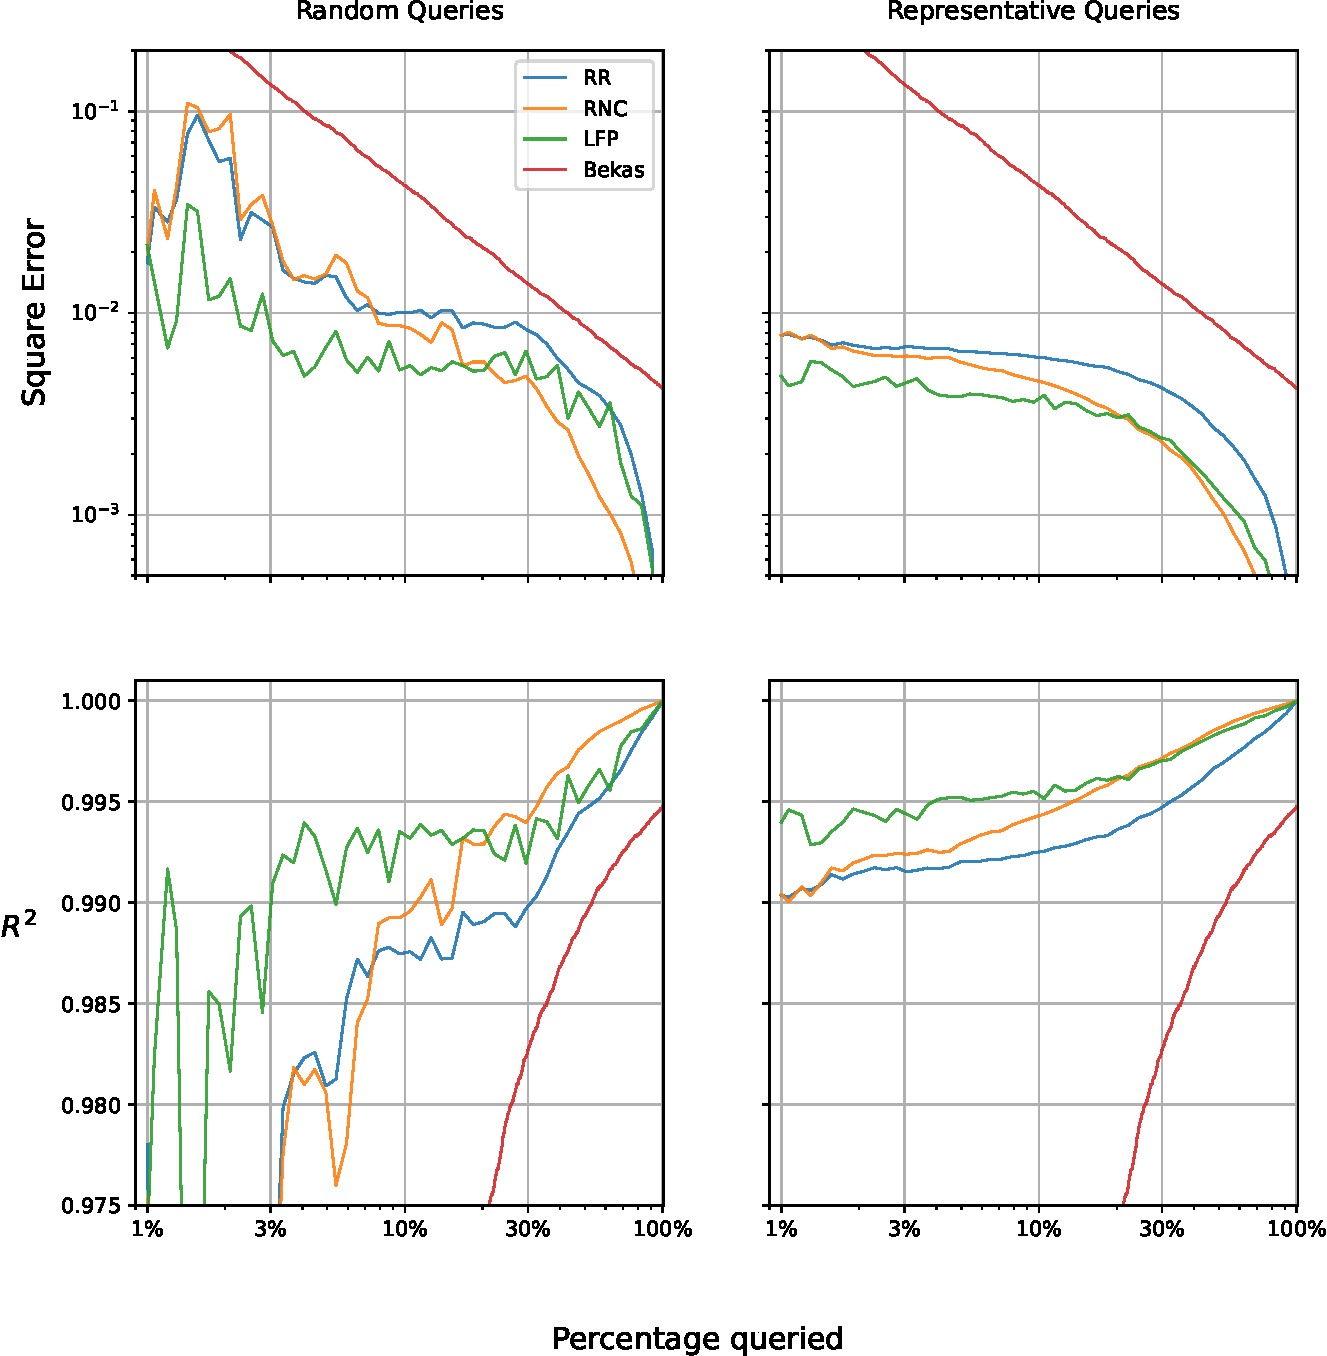
\includegraphics[width=\linewidth]{Figures/VarSolvers.pdf}
    \end{center}
   \caption[Performance of various algorithms for predicting the posterior log-variance]{The performance of the various algorithms for predicting the posterior log-variance is shown as a function of the percentage of $\Omegat$ that has been queried. The top row shows the total square error of the posterior variance, and the bottom row shows the $R^2$ statistic. The left column shows results for random queries and the right column show the results when using representative queries as outlined in \cref{al:K_means}. Since the Bekas technique does not depend on this algorithm, it is repeated in the left and right columns for reference. } 
    \label{fig:var_solvers}
\end{figure} 

The results show that the three supervised learning-based strategies (RR, RNC and LFP) all significantly out-perform Bekas on this synthetic dataset. Moreover, when coupled with the representative sampling strategy of \cref{al:K_means}, all three achieve an $R^2$ statistic of around 0.99 when only 1\% of the elements of $\Omegat$ are queried. These results clearly demonstrate the value of this sampling strategy, especially when the number of queries is low. On this dataset, \cref{al:K_means} has a significant positive impact on performance up to a query percentage of around 3\%, beyond which the difference is less pronounced. 

Of the three supervised learning-based techniques, LFP tends to display the strongest performance at low query percentages, for both random and representative query strategies. RR and RNC have similar performance in this domain, with RNC improving more as the query percentage increases. 

Overall, these results demonstrate that high accuracy predictions ($R^2$ of roughly 0.99) can be achieved for a very low query number relative to the total number of nodes $N$, especially when combined with \cref{al:K_means}. While limited to our graph signal processing models, the supervised learning strategy is clearly more effective than the more general technique of \cite{Bekas2007} on this dataset. 


\section{Posterior Sampling}

\label{sec:sampling}


In this section we move on to the second aim of this chapter, which is to produce an algorithm capable of drawing independent samples directly from the posterior. Let us again begin with the tensor-valued Graph Signal Reconstruction problem. Recall that the posterior distribution is 

\begin{equation}
    \f \, | \, \y \sim \Norm{\PP^{-1} \y}{\PP^{-1}}
\end{equation}

where 

\begin{equation}
    \PP \in \R^{N \times N} = \D_{\St} + \gamma \HH^{-2} = \D_{\St} + \gamma \U \D_\Gt^{-2} \U^\top 
\end{equation}

The most straightforward approach would be to perform Cholesky decomposition directly on the covariance matrix $\PP^{-1}$, such that $\PP^{-1} = \LL \LL^\top$, where $\LL$ is a lower triangular matrix. Every positive-definite matrix (and thus also every valid covariance matrix) has a unique Cholesky decomposition \citep{Horn2012}. Independent samples can then be drawn according to 

\begin{equation}
    \label{eq:post_precision}
    \f_i = \PP^{-1} \y + \LL \z_i
\end{equation}

where $\z_i \in \R^N$ is a random vector with components that are independent standard normal variates which can be generated, for example, by using the Box-Muller transform \citep{Box1958}. Alternatively, if we can perform eigen-decomposition on the covariance matrix into $\PP^{-1} = \U \LAM \U^\top$, then samples can be drawn according to

\begin{equation}
    \f_i = \PP^{-1} \y + \U \LAM^{1/2} \z_i
\end{equation}

Both these techniques assume that the covariance matrix $\PP^{-1}$ can be directly decomposed in a reasonable amount of time. However, in the case of the GSR problem, $\PP^{-1}$ is not directly available. We instead have a representation of $\PP$ in terms of a diagonal and Kronecker structured operator, as given in \cref{eq:post_precision}. For even a modestly-sized GSR problem, this makes these approaches numerically infeasible due to both computational cost and memory footprint. 

\subsection{Perturbation optimization (PO)}

\label{sec:PO}

Perturbation Optimisation (PO) is a technique for sampling from high-dimensional Gaussian distributions when the precision matrix $\PP$ is of the form 

\begin{equation}
    \label{eq:PO_sum}
    \PP = \sum_{k=1}^K \M_k^\top \RR_k^{-1} \M_k
\end{equation}

where $\left\{\RR_k\right\}$ are a set of alternative covariance matrices from which it is easier to draw samples from, and $\left\{\M_k\right\}$ are a set of arbitrary full-rank square matrices \citep{Papandreou2010, Orieux2012}. The PO algorithm gives a method for drawing samples from the distribution $\Norm{\zero}{\PP^{-1}}$, which is achieved by completing the following steps. 

\begin{enumerate}
    \item Step P (Perturbation): For $k$ from 1 to $K$, draw samples $\etaa_k$ from $\Norm{\zero}{\RR_k}$
    \item Step O (Optimisation): Compute $\f$ as the minimiser of the criterion $$J(\f) = \sum_{k=1}^K \left(\etaa_k - \M_k \f \right)^\top \RR_k^{-1}\left(\etaa_k - \M_k \f \right)$$
\end{enumerate}
 
Once the optimisation step has been completed, the resultant vector, $\f$, will be distributed according to $\Norm{\zero}{\PP^{-1}}$. This can be trivially extended to non-centered distributions by adding the mean to the each sample. It's important to note that for PO to be an effective algorithm, it necessitates efficient resolution of the optimisation step. As we will see, in our case we can exploit the Kronecker structure of the relevant matrices to accomplish this step for the same computational cost as computing the mean.  

\subsection{PO for Graph Signal Reconstruction}

\label{sec:GSR_PO}


In the case of graph signal reconstruction, we have that 

$$
\PP = \D_\St + \gamma \U \D_\Gt^{-2} \U^\top
$$

Comparing this to the form required for PO given in \cref{eq:PO_sum}, we can substitute the following values. Note that, since $\D_\St$ is diagonal and binary, $\D_\St^2 = \D_\St$. 

$$
\M_1 = \D_\St, \quad  \RR_1 = \I_N, \quad \M_2 = \sqrt{\gamma} \, \U^\top, \quad  \RR_2 = \D_\Gt^2
$$

The random samples $\etaa_1$ and $\etaa_2$ can be generated by setting $\etaa_1 = \z_1$ and $\etaa_2 = \D_\Gt \z_2$ where $\z_1$ and $\z_2$ are independently drawn from a multivariate standard normal distribution. This gives the following optimisation objective $J(\f)$.

\begin{equation}
    J(\f) = \left(\z_1 - \D_\St \f\right)^\top\left(\z_1 - \D_\St \f\right) + \left(\D_\Gt \z_2 - \sqrt{\gamma} \, \U^\top  \f\right)^\top \D_\Gt^{-2} \left(\D_\Gt \z_2 - \sqrt{\gamma} \, \U^\top  \f\right)
\end{equation}

Taking the derivative with respect to $\f$, setting the result equal to zero, and solving for $\f$ gives

\begin{equation}
    \f = \PP^{-1} \left(\D_\St \z_1 + \sqrt{\gamma} \, \U \D_\Gt^{-1} \z_2 \right)
\end{equation}

This generates random vectors $\f$ distributed according to $\Norm{\zero}{\PP^{-1}}$. To transform this into a distribution with mean $\PP^{-1} \y$, we can simply add this term on. 

\begin{equation}
    \f = \PP^{-1} \left(\y + \D_\St \z_1 + \sqrt{\gamma} \, \U \D_\Gt^{-1} \z_2 \right)
\end{equation}

However, in its current form, the solution presents two issues. Firstly, the multiplication by the matrix $\PP^{-1}$ may result in an ill-conditioned linear system. Secondly, $\z_2$ is multiplied by the matrix $\D_\Gt^{-1}$, which, for certain filters like the bandlimited filter that maps some values to zero, may map some values to infinity. Both problems can be addressed by introducing the symmetric preconditioner $\PSI$ as discussed in \cref{sec:CGM_dd}. As previously stated, this is given by

\begin{equation}
    \PSI = \U \D_\Gt
\end{equation}

This transforms the system into 

\begin{align}
    \f &= \PSI \left(\PSI^\top \PP \PSI \right)^{-1} \PSI^\top \left(\y + \D_\St \z_1 + \sqrt{\gamma} \, \U \D_\Gt^{-1} \z_2 \right) \notag \\
    &= \PSI \Q^{-1} \left(\PSI^\top \y + \PSI^\top \D_\St \z_1 + \sqrt{\gamma} \, \z_2\right)
    \label{eq:PO_sample_GSR}
\end{align}

where 

$$
\Q = \PSI^\top \PP \PSI  = \D_\Gt \U^\top \D_\St \U \D_\Gt + \gamma \I_N 
$$

With this preconditioner in place, the linear system $\Q^{-1} \left(\PSI^\top \y + \PSI^\top \D_\St \z_1 + \sqrt{\gamma} \, \z_2\right)$ can then be solved efficiently using the CGM. For the sake of completeness, we now provide a brief proof that the expression given in \cref{eq:PO_sample_GSR} generates samples from the correct distribution. 

\begin{theorem}
    Consider the following expression for the vector $\f \in \R^N$. 

    $$
    \f = \PSI \Q^{-1} \left(\PSI^\top \y + \PSI^\top \D_\St \z_1 + \sqrt{\gamma} \, \z_2\right)
    $$
    
    If $z_1, z_2 \sim \Norm{\zero}{\I_N}$, then $\f$ is distributed according to
    
    $$
    \f \sim \Norm{\PP^{-1} \y }{\PP^{-1}}
    $$ 

    \label{the:GSR_PO}
\end{theorem}

\begin{proof}
    To prove this statement it suffices to show that the expected value of $\f$ is $\PP^{-1}\y$, and that the covariance is $\PP^{-1}$. Note that the following identities hold. 

    \begin{align*}
        &(a) \;\; \Q = \PSI^\top \PP \PSI, \quad &&(b) \;\; \PP = \PSI^{-\top} \Q \PSI^{-1}, \\
        &(c) \;\; \Q^{-1} = \PSI^{-1} \PP^{-1} \PSI^{-\top}, \quad &&(d) \;\; \PP^{-1} = \PSI \Q^{-1} \PSI^\top
    \end{align*}
    
    Let us begin with the expected value. 

    \begin{equation*}
        \text{E}\left[\f\right] = \text{E}\left[\PSI \Q^{-1} \left(\PSI^\top \y + \PSI^\top \D_\St \z_1 + \sqrt{\gamma} \, \z_2\right)\right]
    \end{equation*}

    Since $\text{E}\left[\z_1\right] = \text{E}\left[\z_2\right] = \zero$, these two terms can be dropped from the expression, leaving 

    \begin{equation*}
        \text{E}\left[\f\right] = \PSI \Q^{-1} \PSI^\top \y
    \end{equation*}

    Making use of identity (d), this is then 

    \begin{equation*}
        \text{E}\left[\f\right] = \PP^{-1} \y
    \end{equation*}

    Next, let us compute the covariance. 

    \begin{equation*}
        \text{Cov}\left[\f\right] = \text{Cov}\left[\PSI \Q^{-1} \left(\PSI^\top \y + \PSI^\top \D_\St \z_1 + \sqrt{\gamma} \, \z_2\right)\right] 
    \end{equation*}

    Consider the three terms within the inner brackets. Since the first has no stochastic component, it does not contribute to the covariance and can therefore dropped. 

    \begin{align*}
        \text{Cov}\left[\f\right] &= \text{Cov}\left[\PSI \Q^{-1} \left(\PSI^\top \D_\St \z_1 + \sqrt{\gamma} \, \z_2\right)\right]  \\
        &= \PSI \Q^{-1} \left(\text{Cov}\left[ \PSI^\top \D_\St \z_1 \right] + \text{Cov}\left[\sqrt{\gamma} \,  \z_2\right]\right) \Q^{-1} \PSI^\top \\
        &= \PSI \Q^{-1} \left(\PSI^\top \D_\St \, \text{Cov}\left[  \z_1 \right] \D_\St \PSI + \gamma \, \text{Cov}\left[ \z_2\right]\right) \Q^{-1} \PSI^\top  \\
        &= \PSI \Q^{-1} \left(\PSI^\top \D_\St \PSI + \gamma \, \I_N \right) \Q^{-1} \PSI^\top  \\
        &= \PSI \Q^{-1} \Q \Q^{-1} \PSI^\top \\
        &= \PSI \Q^{-1} \PSI^\top \\
        &= \PP^{-1}
    \end{align*}

    We have therefore shown that $\text{E}\left[\f\right] = \PP^{-1} \y$ and that $\text{Cov}\left[\f\right] = \PP^{-1}$, completing the proof. 

\end{proof}

Given the expression for $\f$ outlined in \cref{eq:PO_sample_GSR}, we have a straightforward procedure for sampling from the posterior distribution of the GSR model, as detailed in \cref{al:PO_GSR}. It's important to note that the primary computational load of this algorithm stems from solving the linear system using the CGM. Consequently, the computational complexity of drawing a single sample from the posterior distribution is equivalent to solving one linear system via the CGM.

\vspace{0.5cm}

\begin{algorithm}[h]
    \begin{algorithmic}
    \vspace{0.15cm}
    \State{Sample $\z_1$ from $\Norm{\zero}{\I_N}$}
    \vspace{0.15cm}
    \State{Sample $\z_2$ from $\Norm{\zero}{\I_N}$}
    \vspace{0.15cm}
    \State{$\aaa \leftarrow \D_\Gt \U^\top \D_\St \z_1 $}
    \vspace{0.15cm}
    \State{$\bb \leftarrow \sqrt{\gamma} \, \z_2$}
    \vspace{0.15cm}
    \State{$\cc \leftarrow \aaa + \bb$}
    \vspace{0.15cm}
    \State{$\PSI \leftarrow \U \D_\Gt$}
    \vspace{0.15cm}
    \State{$\Q \leftarrow  \D_\Gt \U^\top \D_\St \U \D_\Gt + \gamma \I_N $}
    \vspace{0.15cm}
    \State{$\f \leftarrow \Q^{-1} \left(\PSI^\top \y + \cc \right) \quad $ (solve with the CGM)}
    \vspace{0.15cm}
    \State{$\f \leftarrow \PSI \f $}
    \vspace{0.15cm}
    \Ensure{$ \f $}
    \end{algorithmic}
    \caption{Draw one sample from the GSR posterior distribution}
    \label{al:PO_GSR}
\end{algorithm}

\subsection{Drawing samples for KGR, RNC and KG-RNC}

So far in this section, we have shown how perturbation optimisation can be used to draw samples from the posterior distribution of the GSR model. Using the same basic strategy, we can also derive algorithms for the KGR, RNC and KG-RNC models. 

\subsubsection{PO with KGR}

\label{sec:PO_KGR}

In the case of Kernel Graph Regression (KGR), there is little change from the GSR algorithm. Recall how, as discussed in \cref{sec:KGR_and_GSR}, KGR bares a strong algebraic correspondence to GSR. In particular, the posterior distribution over the underlying graph signal $\f$ is given by 

\begin{equation}
    \f \sim \Norm{\bar{\PP}^{-1} \y}{\bar{\PP}^{-1}}
\end{equation}

where 

\begin{equation}
    \bar{\PP} = \D_\St + \gamma \bar{\U} \D_{\bar{\Gt}}^{-2} \bar{\U}^\top
\end{equation}

The values for $\bar{\U}$ and $\D_{\bar{\Gt}}$ are modified from the GSR model as follows. 

\begin{equation}
    \bar{\U} = \V \otimes \U, \aand \D_{\bar{\Gt}} = \diag{\vecrm{\bar{\Gt}}}
\end{equation}

with the elements of $\Gt$ given by 

\begin{equation}
    \Gt_{[t, \nn]} = g\big(\lambdaa(\nn); \, \betaa\big) \sqrt{\lambda^{(K)}_t} 
\end{equation}

With these modifications in place, we can make use of the same algorithm developed in \cref{sec:GSR_PO}, since all the derivations otherwise remain the same. Therefore, in order to sample from the posterior distribution of the KGR model, we can simply reuse \cref{al:PO_GSR}, replacing all instances of $\U$ with $\bar{\U}$, and all instances of $\D_\Gt$ with $\D_{\bar{\Gt}}$. 

\subsubsection{PO with RNC}

\label{sec:PO_RNC}

In the case of Regression with Network Cohesion (RNC), the algorithm must be adjusted. Here, the relevant posterior distribution is over the parameter vector $\thetaa$, rather than the predicted signal $\f$. This posterior distribution is given by 

\begin{equation}
    \thetaa \sim \Norm{\widetilde{\PP}^{-1} \begin{bmatrix} \y \\ \X^\top \y \end{bmatrix}}{\widetilde{\PP}^{-1}}
\end{equation}

where 

\begin{equation}
    \widetilde{\PP} \in \R^{(N + M) \times (N + M)}= 
    \begin{bmatrix}
     \D_\St + \gamma \U \D_\Gt^{-2} \U^\top & \D_\St  \X \\
     \X^\top \D_\St & \X^\top \D_\St \X + \lambda \I_M   
    \end{bmatrix}
\end{equation}

Recall that we can perform eigendecomposition on the matrix $\X^\top\D_\St \X$ as 

$$
\X^\top\D_\St \X = \U_M \LAM_M \U_M^\top
$$

and additionally define the diagonal matrix $\D_M $ as

$$
\D_M = \big(\LAM_M + \lambda \I_M \big)^{-1/2}
$$

Recall also, that the preconditioner used in the case of RNC is 

$$
\widetilde{\PSI} = \begin{bmatrix}
    \U \D_\Gt & \zero \\
    \zero & \U_M \D_M 
\end{bmatrix}
$$

We now present the expression that can be used to sample from the posterior distribution of $\thetaa$ in \cref{the:RNC_PO}.

\begin{theorem}

    Consider the following expression for the vector $\thetaa \in \R^{N + M}$

    \begin{equation}
        \thetaa = \widetilde{\PSI} \widetilde{\Q}^{-1} \left(\widetilde{\PSI}^\top \begin{bmatrix} \y \\ \X^\top \y \end{bmatrix} + \begin{bmatrix}
            \D_\Gt \U^\top \D_\St & \zero \\
            \D_M \U_M^\top \X^\top \D_\St & \zero
        \end{bmatrix} \z_1 + \begin{bmatrix}
            \sqrt{\gamma} \, \I_N & \zero \\
            \zero & \sqrt{\lambda} \D_M
        \end{bmatrix} \z_2 \right)
        \label{eq:PO_sample_RNC}
    \end{equation}

    where the matrix $\widetilde{\Q}$ is given by 

    $$
    \widetilde{\Q} = \widetilde{\PSI}^\top \widetilde{\PP} \widetilde{\PSI}  = \begin{bmatrix}
        \D_\Gt \U^\top \D_\St \U \D_\Gt + \gamma \I_{N}  &  \D_\Gt \U^\top \D_\St \X \U_M \D_M \\[0.1cm] 
        \D_M \U_M^\top \X^\top \D_\St \U \D_\Gt & \I_M
        \end{bmatrix}
    $$

    If $z_1, z_2 \sim \Norm{\zero}{\I_{(N+M)}}$, then
    
    $$
    \thetaa \sim \Norm{\widetilde{\PP}^{-1} \begin{bmatrix} \y \\ \X^\top \y \end{bmatrix}}{\widetilde{\PP}^{-1}}
    $$ 
    
    \label{the:RNC_PO}
\end{theorem}

\begin{proof}
As in \cref{the:GSR_PO}, it suffices to show that

$$
\E\left[\thetaa\right] = \widetilde{\PP}^{-1} \begin{bmatrix} \y \\ \X^\top \y \end{bmatrix}, \aand \text{Cov}\left[\thetaa  \right] = \widetilde{\PP}^{-1} 
$$

Note that the following identities hold. 

    \begin{align*}
        &(a) \;\; \widetilde{\Q} = \widetilde{\PSI}^\top \widetilde{\PP} \widetilde{\PSI}, \quad &&(b) \;\; \widetilde{\PP} = \widetilde{\PSI}^{-\top} \widetilde{\Q} \widetilde{\PSI}^{-1}, \\
        &(c) \;\; \widetilde{\Q}^{-1} = \widetilde{\PSI}^{-1} \widetilde{\PP}^{-1} \widetilde{\PSI}^{-\top}, \quad &&(d) \;\; \widetilde{\PP}^{-1} = \widetilde{\PSI} \widetilde{\Q}^{-1} \widetilde{\PSI}^\top
    \end{align*}

First, let us consider the expected value. Since $\E\left[\z_1\right] = \E\left[\z_2\right] = \zero$, these terms do not contribute to the expected value of $\thetaa$. Therefore, $\E\left[\thetaa\right]$ is given by 

\begin{align*}
    \E\left[\thetaa\right] &= \E\left[\widetilde{\PSI} \widetilde{\Q}^{-1} \widetilde{\PSI}^\top \begin{bmatrix} \y \\ \X^\top \y \end{bmatrix}\right] \\
    &= \widetilde{\PP}^{-1} \begin{bmatrix} \y \\ \X^\top \y \end{bmatrix} 
\end{align*}

For the covariance, let us consider each of the three terms within the brackets of \cref{eq:PO_sample_RNC} in isolation. Since the first term has no stochastic component, the covariance of this is zero. For the second term, the covariance is given by 

\begin{align*}
    \text{Cov}\left[\begin{bmatrix}
        \D_\Gt \U^\top \D_\St & \zero \\
        \D_M \U_M^\top \X^\top \D_\St & \zero
    \end{bmatrix} \z_1 \right] &= \begin{bmatrix}
        \D_\Gt \U^\top \D_\St & \zero \\
        \D_M \U_M^\top \X^\top \D_\St & \zero
    \end{bmatrix} \text{Cov}\left[ \z_1 \right] \begin{bmatrix}
        \D_\Gt \U^\top \D_\St & \zero \\
        \D_M \U_M^\top \X^\top \D_\St & \zero
    \end{bmatrix}^\top \\[0.3cm]
    &= \begin{bmatrix}
        \D_\Gt \U^\top \D_\St & \zero \\
        \D_M \U_M^\top \X^\top \D_\St & \zero
    \end{bmatrix} \begin{bmatrix}
        \D_\St \U \D_\Gt  &  \D_\St \X \U_M \D_M  \\
         \zero  & \zero
    \end{bmatrix} \\[0.3cm]
    &= \begin{bmatrix}
        \D_\Gt \U^\top \D_\St \U \D_\Gt  &  \D_\Gt \U^\top \D_\St \X \U_M \D_M \\[0.1cm] 
        \D_M \U_M^\top \X^\top \D_\St \U \D_\Gt & \D_M \U_M^\top \X^\top \D_\St \X \U_M \D_M 
        \end{bmatrix} \\[0.3cm]
    &= \begin{bmatrix}
        \D_\Gt \U^\top \D_\St \U \D_\Gt  &  \D_\Gt \U^\top \D_\St \X \U_M \D_M \\[0.1cm] 
        \D_M \U_M^\top \X^\top \D_\St \U \D_\Gt & \D_M \LAM_M \D_M 
        \end{bmatrix} \\
\end{align*}

Now consider the covariance of the third term. 

\begin{align*}
    \text{Cov}\left[\begin{bmatrix}
        \sqrt{\gamma} \, \I_N & \zero \\
        \zero & \sqrt{\lambda} \D_M
    \end{bmatrix} \z_2  \right] &= \begin{bmatrix}
        \sqrt{\gamma} \, \I_N & \zero \\
        \zero & \sqrt{\lambda} \D_M
    \end{bmatrix}  \text{Cov}\left[ \z_2 \right] \begin{bmatrix}
        \sqrt{\gamma} \, \I_N & \zero \\
        \zero & \sqrt{\lambda} \D_M
    \end{bmatrix} \\[0.3cm]
    &= \begin{bmatrix}
        \gamma\, \I_N & \zero \\
        \zero & \lambda \D_M^2
    \end{bmatrix}
\end{align*}

Note that these two matrices summed together give 

\begin{align*}
    & \begin{bmatrix}
        \D_\Gt \U^\top \D_\St \U \D_\Gt  &  \D_\Gt \U^\top \D_\St \X \U_M \D_M \\[0.1cm] 
        \D_M \U_M^\top \X^\top \D_\St \U \D_\Gt & \D_M \LAM_M \D_M 
        \end{bmatrix} + \begin{bmatrix}
            \gamma\, \I_N & \zero \\
            \zero & \lambda \D_M^2
        \end{bmatrix} \\[0.3cm]
        &= \begin{bmatrix}
            \D_\Gt \U^\top \D_\St \U \D_\Gt  + \gamma\, \I_N &  \D_\Gt \U^\top \D_\St \X \U_M \D_M \\[0.1cm] 
            \D_M \U_M^\top \X^\top \D_\St \U \D_\Gt & \D_M \LAM_M \D_M + \lambda \D_M^2
            \end{bmatrix} \\[0.3cm]
        &= \begin{bmatrix}
            \D_\Gt \U^\top \D_\St \U \D_\Gt  + \gamma\, \I_N &  \D_\Gt \U^\top \D_\St \X \U_M \D_M \\[0.1cm] 
            \D_M \U_M^\top \X^\top \D_\St \U \D_\Gt & \I_M
            \end{bmatrix} \\[0.3cm]
        &= \widetilde{\Q}
\end{align*}

Note that here we have used the fact that $\D_M \LAM_M \D_M + \lambda \D_M^2 = \I_M$. This is true since 

\begin{align*}
    \D_M \LAM_M \D_M + \lambda \D_M^2 &= \LAM_M \D_M^2 + \lambda \D_M^2 \\
    &= (\LAM_M + \lambda \I_M) \D_M^2 \\
    &= \D_M^{-2}  \D_M^2 \\
    &= \I_M
\end{align*}

Therefore, the covariance of the entire expression is given by 

\begin{align*}
    \text{Cov}\left[\thetaa\right] &= \widetilde{\PSI} \widetilde{\Q}^{-1} \widetilde{\Q} \widetilde{\Q}^{-1} \widetilde{\PSI}^\top \\
    &= \widetilde{\PSI} \widetilde{\Q}^{-1} \widetilde{\PSI}^\top  \\
    &= \widetilde{\PP}^{-1}
\end{align*}

We have therefore shown that 

$$
\E\left[\thetaa\right] = \widetilde{\PP}^{-1} \begin{bmatrix} \y \\ \X^\top \y \end{bmatrix}, \aand \text{Cov}\left[\thetaa  \right] = \widetilde{\PP}^{-1} 
$$

completing the proof. 

\end{proof}


Given this expression for $\thetaa$ stated in \cref{eq:PO_sample_RNC}, a simple procedure for sampling from the posterior distribution of the RNC model is available. This is given in \cref{al:PO_RNC}. 

\begin{algorithm}[h]
    \begin{algorithmic}
    \vspace{0.15cm}
    \State{Sample $\z_1$ from $\Norm{\zero}{\I_{(N + M)}}$}
    \vspace{0.15cm}
    \State{Sample $\z_2$ from $\Norm{\zero}{\I_{(N + M)}}$}
    \vspace{0.25cm}
    \State{$\aaa \leftarrow \begin{bmatrix}
        \D_\Gt \U^\top \D_\St & \zero \\
        \D_M \U_M^\top \X^\top \D_\St & \zero
    \end{bmatrix} \z_1  $}
    \vspace{0.25cm}
    \State{$\bb \leftarrow \begin{bmatrix}
        \sqrt{\gamma} \, \I_N & \zero \\
        \zero & \sqrt{\lambda} \D_M
    \end{bmatrix} \z_2$}
    \vspace{0.25cm}
    \State{$\cc \leftarrow \aaa + \bb$}
    \vspace{0.25cm}
    \State{$\PSI \leftarrow \begin{bmatrix}
        \U \D_\Gt & \zero \\
        \zero & \U_M \D_M 
    \end{bmatrix}$}
    \vspace{0.25cm}
    \State{$\Q \leftarrow  \begin{bmatrix}
        \D_\Gt \U^\top \D_\St \U \D_\Gt  + \gamma\, \I_N &  \D_\Gt \U^\top \D_\St \X \U_M \D_M \\[0.1cm] 
        \D_M \U_M^\top \X^\top \D_\St \U \D_\Gt & \I_M
        \end{bmatrix}  $}
    \vspace{0.25cm}
    \State{$\thetaa \leftarrow \Q^{-1} \left(\PSI^\top \begin{bmatrix} \y \\ \X^\top \y \end{bmatrix} + \cc \right) \quad $ (solve with the CGM)}
    \vspace{0.25cm}
    \State{$\thetaa \leftarrow \PSI \thetaa $}
    \vspace{0.25cm}
    \Ensure{$ \thetaa $}
    \end{algorithmic}
    \caption{Draw one sample from the RNC posterior distribution}
    \label{al:PO_RNC}
\end{algorithm}


\subsubsection{PO with KG-RNC}

\label{sec:PO_KGRNC}

For the case of Kernel Graph Regression with Network Cohesion (KG-RNC), the situation is algebraically very similar to that of RNC. Just as the algorithm for sampling from the KGR model posterior can be obtained by making a small modification to the GSR case as discussed in \cref{sec:PO_KGR}, the same is true of KG-RNC, with only a small modification of the RNC algorithm. In particular, the posterior distribution over the parameter vector $\hat{\thetaa}$ is given by 

\begin{equation}
    \label{eq:KGRNC_post_PO}
    \hat{\thetaa} \sim \mathcal{N}\left(\hat{\PP}^{-1} \begin{bmatrix} \y \\ \X^\top \y \end{bmatrix}, \, \hat{\PP}^{-1}\right)
\end{equation}

where 

\begin{equation}
    \hat{\PP} \in \R^{(N + M) \times (N + M)}= 
    \begin{bmatrix}
     \D_\St + \gamma \bar{\U} \D_{\bar{\Gt}}^{-2} \bar{\U}^\top & \D_\St  \X \\
     \X^\top \D_\St & \X^\top \D_\St \X + \lambda \I_M   
    \end{bmatrix}
\end{equation}

Note that this is the same posterior distribution as in the RNC model, with the objects $\U$ and $\Gt$ replaced by $\bar{\U}$ and $\bar{\Gt}$. These have the same values as in \cref{sec:PO_KGR}. In particular

\begin{equation}
    \bar{\U} = \V \otimes \U, \aand \D_{\bar{\Gt}} = \diag{\vecrm{\bar{\Gt}}}
\end{equation}

with the elements of $\Gt$ given by 

\begin{equation}
    \Gt_{[t, \nn]} = g\big(\lambdaa(\nn); \, \betaa\big) \sqrt{\lambda^{(K)}_t} 
\end{equation}

Therefore, in order to draw samples from the distribution given in \cref{eq:KGRNC_post_PO}, we can simply reuse \cref{al:PO_RNC}, replacing every instance of $\U$ with $\bar{\U}$ and every instance of $\Gt$ with $\bar{\Gt}$. 

\section{Variance Estimation: Prediction vs Sampling}

\label{sec:comparison}

So far in this chapter we have addressed estimation of the posterior marginal variance and direct sampling from the posterior as separate objectives. In \cref{sec:post_var_pred}, we proposed several methods based on a supervised learning approach, aiming to predict the entire marginal variance (i.e., the diagonal of the posterior covariance matrix), given our ability to ``query" a subset of these matrix elements. On the other hand, in \cref{sec:sampling}, we developed methods for direct sampling from the posterior. However, it's evident that a valid approach to estimating the marginal variance would be to simply draw samples, using the techniques discussed in \cref{sec:sampling}, and compute the sample variance as an estimator for the population variance. This naturally raises the question of whether this approach is superior to the supervised learning approaches discussed in \cref{sec:post_var_pred}. 

Let us take the Graph Signal Reconstruction model as the primary example. If we have already computed the posterior mean, $\f^\star = \PP^{-1}\y$, then an unbiased estimator for the posterior marginal variance based on $K$ samples $\{\f_k\}_{k=1}^K$ is clearly

\begin{equation}
    \sigmaa^2_K = \frac{1}{K} \sum_{k=1}^K (\f_k - \f^\star)^2
\end{equation}

where the exponent is understood as element-wise. In order not to hold all $K$ samples in memory simultaneously, we can write this in recursive form as 

\begin{equation}
    \sigmaa^2_{K+1} = \frac{1}{K + 1} \left( K \sigmaa^2_K  + (\f_{k+1} - \f^\star)^2\right)
\end{equation}

The relative error of this estimator follows from the properties of the $\chi^2$ distribution, and is thus given by 

\begin{equation}
    r = \sqrt{\frac{2}{K}}
\end{equation}

meaning $K = 2 / r^2$ samples are necessary to reduce the relative error to a fraction $r$. For example, 50 samples would be required to reduce the relative error to $20\%$. However, one attractive feature of this estimator is that its accuracy is independent of the size of the graph. Whether this is also the case for the supervised learning estimators is not immediately clear. 

\subsection{Experiments}

In order to investigate the properties of these two approaches to estimating the posterior marginal variance, that is, the supervised learning approaches discussed in \cref{sec:post_var_pred}, and the sample variance approach highlighted in \cref{sec:comparison}, we ran the following experiment. Graphs, comprising the Cartesian product of three random fully-connected sub-graphs, were created in increasing size. For each, we generated a random pattern of missingness $\St$ by uniformly sampling each element from $\{0, 1\}$, and tested the three supervised learning approaches (with active learning), the Bekas diagonal estimator, and the sample-based approach for predicting the posterior marginal variance. As with the experiments in \cref{sec:logvar_experiments}, we used a diffusion filter with $\betaa = [0.5, 0.7, 0.6]$ and set $\gamma=1$. Each estimator was given a budget of 50 linear system solves, and its prediction performance was measured by the $R^2$ score. The result are show in \cref{fig:var_comparison}.


\begin{figure}[t] 
    \begin{center}
        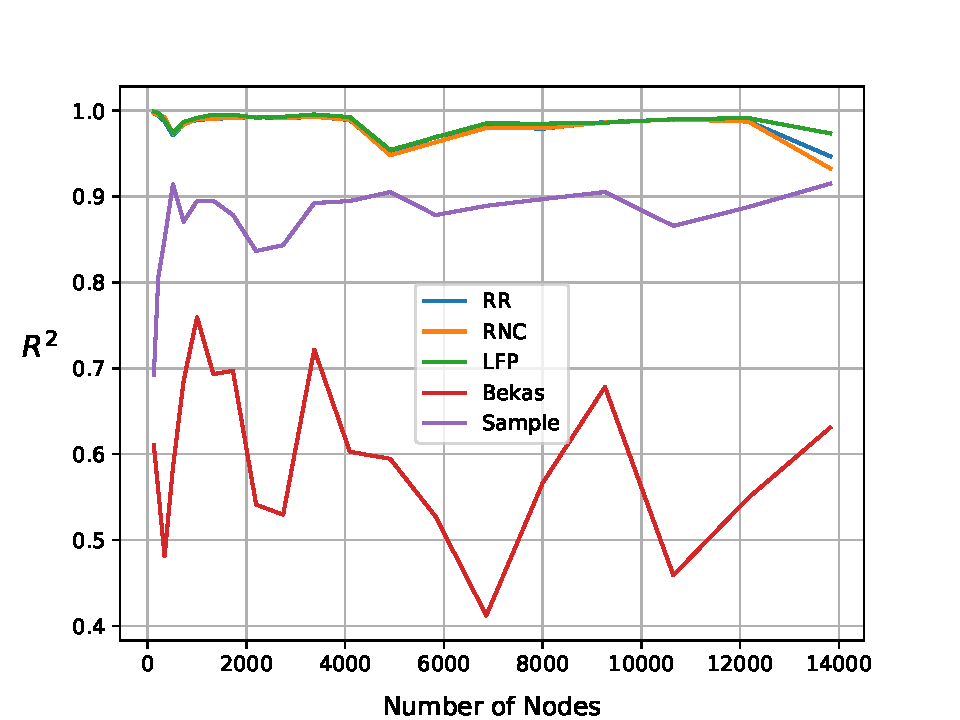
\includegraphics[width=0.8\linewidth]{Figures/sample_diag_estimation.pdf}
    \end{center}
   \caption[Performance of the sampling strategy for predicting posterior marginal variance compared with the supervised learning strategies as a function of graph size]{The predictive performance, as measured by $R^2$, is shown for the three supervised learning strategies detailed in \cref{sec:logvar_supervised}, the Bekas diagonal estimator of \cref{sec:logvar_bekas}, and the sampling strategy of \cref{sec:comparison}. } 
    \label{fig:var_comparison}
\end{figure} 


As visible, RR, RNC and LFP all have similar performance over the range of graph sizes, with $R^2$ never dropping below 0.9. Of the three, LFP once again achieves the highest accuracy, although the difference compared to RR and RNC is fairly small. The sample-based estimator achieves an $R^2$ of around 0.85-0.9 across the range of graph sizes, with performance dropping as low as 0.7 but mostly remaining within this bound. Its performance is also between that of the Bekas diagonal estimator and the three supervised learning techniques over the whole range. 

While the supervised learning estimators are fairly consistent, there is some evidence that their performance is dropping as node number increases. Unfortunately, it is difficult to test this hypothesis since, in order to tets the accuracy scores, it is necessary to solve for the entire posterior variance meaning the number of linear system solves required to run this experiment increases rapidly as the number of nodes increases. 

\section{Conclusions}

In this chapter, we have presented a detailed examination of various methods related to the posterior covariance of the tensor GSP models introduced in \cref{chap:nd_gsp}. In the case of GSR, KGR, RNC and KG-RNC, the posterior distribution is a high-dimensional Gaussian with a precision matrix, $\PP$, characterised by Kronecker-structured operators. The implicit dimensionality of $\PP$ makes direct decomposition and inversion operations challenging, necessitating the use of computationally efficient techniques that avoid the time and memory costs associated with more straightforward approaches.

We concentrated on two distinct tasks. First, in \cref{sec:post_var_pred}, we aimed to estimate the posterior marginal variance, i.e. the diagonal of $\SIG = \PP^{-1}$. In particular, we compared a recent stochastic algorithm devised by \cite{Bekas2007} against three supervised learning-based techniques. This was achieved by first noting that it is possible to compute (or ``query'') a subset of the elements of $\PP^{-1}$ directly by solving the linear system $\PP^{-1} \e_n$, where $\e_n$ is a unit basis vector. Next, by creating a set of artificial explanatory variables associated with each element, the task of estimating the non-queried elements was framed in terms of a traditional supervised learning task. We proposed three separate estimators, namely Ridge Regression (RR), Regression with Network Cohesion (RNC), and Learned Filter Parameters (LFP), for prediction. On a synthetic dataset, all three were capable of achieving high accuracy ($R^2 > 0.99$) for a small fraction of the computational cost of computing the marginal variance in full. We also combined this with an active learning strategy which increased prediction accuracy further, especially at low query numbers.  

In \cref{sec:sampling}, we focused on the task of drawing samples directly from the posterior distribution. To achieve this, we made use of a technique known as Perturbation Optimisation (PO) \citep{Orieux2012}, which takes advantage of the special structure of the posterior precision matrix  to reduce the computational cost to one linear system solve per sample. By coupling this with the symmetric preconditioner $\PSI$, we were able to remedy the numerical difficulties associated with the algorithm in its basic form to produce an efficient procedure using the CGM. We demonstrated that this procedure yielded the correct posterior distribution for the GSR, RNC, KGR, and KG-RNC algorithms in their general tensor form.  

Finally, in \cref{sec:comparison}, we explored whether the sampling algorithm developed in \cref{sec:sampling} could serve as an alternative method for estimating the posterior marginal variance. By assessing the prediction accuracy over product graphs of increasing size, we found that the supervised learning techniques typically outperform the sampling strategy. However, for very large graphs, sampling may be preferable, as the relative error is independent of the graph's size, while the supervised learning techniques show some signs of performance degradation as the number of nodes grows. Further research into this question would be valuable.